\documentclass[letterpaper,9pt,twocolumn,twoside,]{pinp}

%% Some pieces required from the pandoc template
\providecommand{\tightlist}{%
  \setlength{\itemsep}{0pt}\setlength{\parskip}{0pt}}

% Use the lineno option to display guide line numbers if required.
% Note that the use of elements such as single-column equations
% may affect the guide line number alignment.

\usepackage[T1]{fontenc}
\usepackage[utf8]{inputenc}

% pinp change: the geometry package layout settings need to be set here, not in pinp.cls
\geometry{layoutsize={0.95588\paperwidth,0.98864\paperheight},%
  layouthoffset=0.02206\paperwidth, layoutvoffset=0.00568\paperheight}

\definecolor{pinpblue}{HTML}{185FAF}  % imagecolorpicker on blue for new R logo
\definecolor{pnasbluetext}{RGB}{101,0,0} %


\usepackage{float} \floatplacement{figure}{h} \usepackage{fancyhdr} \pagestyle{fancy} \fancyfoot{}

\title{Predictive modelling of weight at birth}

\author[]{Flynn Entwistle, Jerry Shum, Lara Pierce, Shaun Lim, Eric
Huang}


\setcounter{secnumdepth}{0}

% Please give the surname of the lead author for the running footer
\leadauthor{Author and Author}

% Keywords are not mandatory, but authors are strongly encouraged to provide them. If provided, please include two to five keywords, separated by the pipe symbol, e.g:
 

\begin{abstract}
We sought to analyse the significance of 8 variables as predictors of
weight at birth in a multiple regression model, using observations
collected from Baystate Medical Centre, MA (n=189). A supplementary
investigation also took place to compare out of sample performance
between models trained on the original presentation of categorical
variables, and an alternative dataset where factor levels with few
observations had been merged. 6 of the studied variables were found to
be significant predictors of birth weight, with merged factor levels in
the case of few observations providing the best out of sample
performance.
\end{abstract}

\dates{This version was compiled on \today} 


% initially we use doi so keep for backwards compatibility
% new name is doi_footer


\begin{document}

% Optional adjustment to line up main text (after abstract) of first page with line numbers, when using both lineno and twocolumn options.
% You should only change this length when you've finalised the article contents.
\verticaladjustment{-2pt}

\maketitle
\thispagestyle{firststyle}
\ifthenelse{\boolean{shortarticle}}{\ifthenelse{\boolean{singlecolumn}}{\abscontentformatted}{\abscontent}}{}

% If your first paragraph (i.e. with the \dropcap) contains a list environment (quote, quotation, theorem, definition, enumerate, itemize...), the line after the list may have some extra indentation. If this is the case, add \parshape=0 to the end of the list environment.


\pagestyle{fancy}
\fancyfoot{}
\small

\section{Introduction}\label{introduction}

Low birth weight expresses comorbidity with a broad range of health
complications among infants, shown to be prevalent in 15-20\% of newborn
mortality cases worldwide, and a predictor for stunting and other
metabolic risk factors in later life
(\href{https://pubmed.ncbi.nlm.nih.gov/3880598/}{McCormick, 1985}). But
despite its effects being well documented in the current scientific
literature, predictors of low birth weight during pregnancy remain
scarcely considered. Addressing this deficit, we sought to find the most
significant predictors of low birth weight. Multiple regression models
were constructed for this purpose, before choosing one which optimised
for out of sample performance to increase the how well our model
generalised to future observations. Future investigations should
consider how well the findings of this study generalise to predict birth
weight within a more diverse sample - between different hospitals and
regions.

\subsection{Discussion of data}\label{discussion-of-data}

The \texttt{birthwt} dataset obtained from the \texttt{MASS} package
contains observations from \((n=189)\) mothers collected in 1986 at
Baystate Medical Centre in Springfield, Massachusetts. The dataset
contained 10 variables in total. For the purposes of this study, we took
infant birth weight as the dependent variable. \texttt{low} provided no
useful information in predicting birth weight, so was dropped from the
dataset. This left 4 numerical and 4 categorical independent variables
which we could investigate as predictors of birth weight. Studied
variables were renamed and transformed to metric units for legibility
and ease of comparison. \href{tba1}{Table A1} contains a tabular summary
of the dataset.

\section{Analysis}\label{analysis}

\subsection{Preliminary
transformations}\label{preliminary-transformations}

From our EDA, we knew some predictors to individually not satisfy our
assumptions with respect to the dependent variable.

\begin{ShadedResult}
\begin{verbatim}
#  Warning: The dot-dot notation (`..rr.label..`) was deprecated in ggplot2 3.4.0.
#  i Please use `after_stat(rr.label)` instead.
#  This warning is displayed once every 8 hours.
#  Call `lifecycle::last_lifecycle_warnings()` to see where this warning was
#  generated.
\end{verbatim}
\end{ShadedResult}
\begin{figure}

{\centering 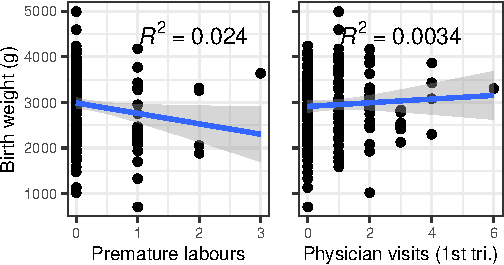
\includegraphics{Executive-Summary_files/figure-latex/fig1-1} 

}

\caption{Premature labours and first trimester physician visits against birth weight (numerical)}\label{fig:fig1}
\end{figure}

\href{fig1}{Figure 1} shows the discrete numerical variables
\emph{number of premature labours} and \emph{first trimester physician
visits} to each have too few intervals to confidently suggest a linear
relationship.

No mathematical transformations would be appropriate here. But, rather
than dropping these variables from the model, their few unique values
allowed us to reasonably transform them into categorical variables as
per \href{fig2}{Figure 2} \small

\begin{Shaded}
\begin{Highlighting}[]
\NormalTok{birthwt}\SpecialCharTok{$}\NormalTok{Premature\_labours }\SpecialCharTok{\%\textless{}\textgreater{}\%} \FunctionTok{factor}\NormalTok{()}
\NormalTok{birthwt}\SpecialCharTok{$}\NormalTok{First\_tri\_physician\_visits }\SpecialCharTok{\%\textless{}\textgreater{}\%} \FunctionTok{factor}\NormalTok{()}
\end{Highlighting}
\end{Shaded}

\begin{figure}

{\centering 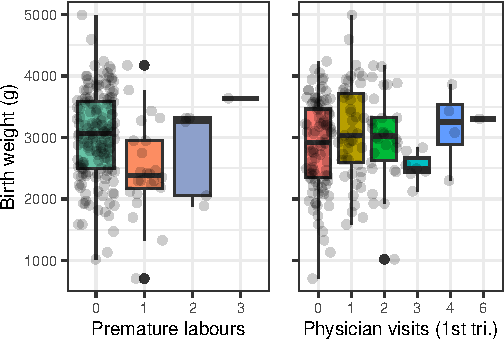
\includegraphics{Executive-Summary_files/figure-latex/fig1.5-1} 

}

\caption{Premature labours and first trimester physician visits against birth weight (factored)}\label{fig:fig1.5}
\end{figure}

Additionally, it was found that when applying a log transformation to
\emph{weight at last menstruation}, linearity and homoscedascity
assumptions were more confidently satisfied against the dependent
variable, with a more uniform spread of residuals above and below 0 when
plotting against fitted values.

\small

\begin{Shaded}
\begin{Highlighting}[]
\NormalTok{birthwt }\SpecialCharTok{\%\textless{}\textgreater{}\%} \FunctionTok{mutate}\NormalTok{(log\_weight\_at\_last\_menstruation}
           \OtherTok{=} \FunctionTok{log}\NormalTok{(Weight\_at\_last\_menstruation))}
\end{Highlighting}
\end{Shaded}

\subsection{\texorpdfstring{Alternative dataset with merged \texttt{ptl}
and \texttt{ftv}
levels}{Alternative dataset with merged ptl and ftv levels}}\label{alternative-dataset-with-merged-ptl-and-ftv-levels}

Factorising premature labours and first trimester physician visits
allowed our linearity assumptions to be met, but created some levels
with very few observations \((n\leq 5)\).

We hypothesised that this could be a source of overfitting -
unnecessarily complicating our model with extra predictors whilst
providing unreliable information about the dependent variable at these
levels.

To test for this, we created an alternative dataset where levels with
few observations in these variables had been merged together as per
\href{tab1}{Table 1}.

\begin{table}[h]
\begin{minipage}{.28\textwidth}
  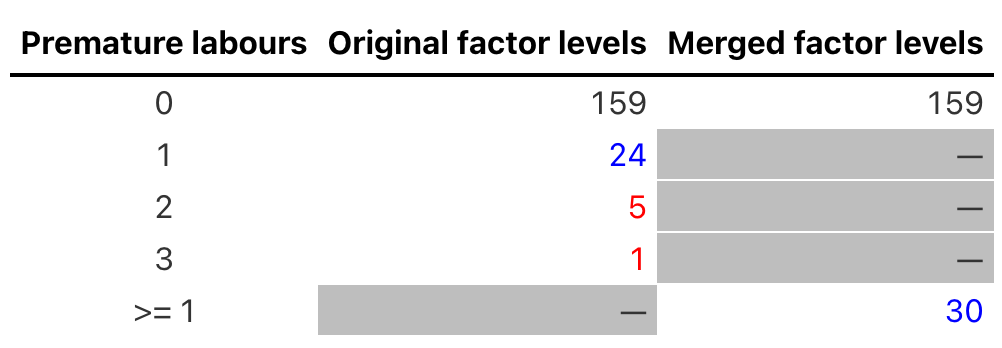
\includegraphics[width=\textwidth, height = 2.65cm]{ptltab}
\end{minipage}%
\begin{minipage}{0.3\textwidth}
  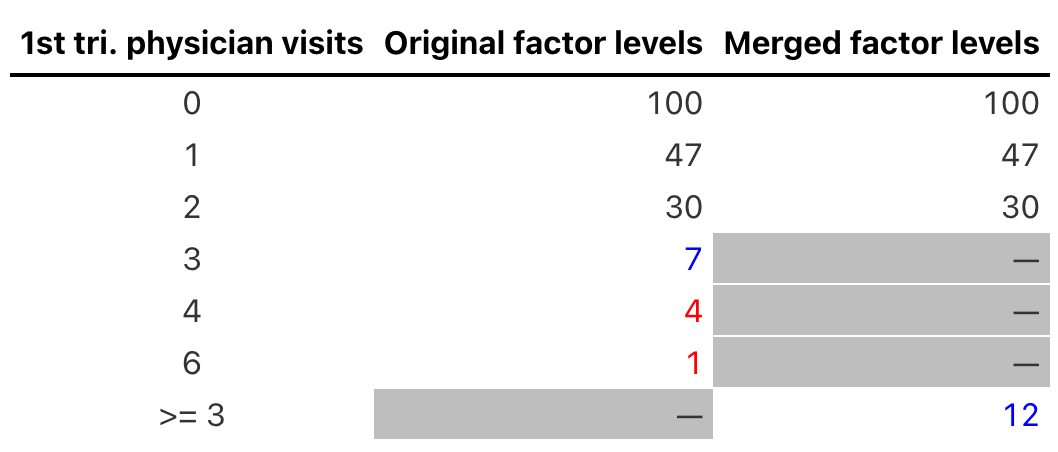
\includegraphics[width=\textwidth, height = 2.75cm]{ftvtab}
\end{minipage}%
\caption{Level merging - Premature labours (left) and First trimester physician visits (right)}
\end{table}

These will be analysed in comparison with models trained on the original
presentation of these factors.

\subsection{Post-transformation assumption
checking}\label{post-transformation-assumption-checking}

After transformation, we constructed full models for both datasets
incorporating all variables as predictors of birth weight.

\small

\begin{Shaded}
\begin{Highlighting}[]
\NormalTok{M1.original }\OtherTok{\textless{}{-}} \FunctionTok{lm}\NormalTok{(Birth\_weight }\SpecialCharTok{\textasciitilde{}}\NormalTok{ ., }\AttributeTok{data=}\NormalTok{birthwt)}
\NormalTok{M1.merged }\OtherTok{\textless{}{-}} \FunctionTok{lm}\NormalTok{(Birth\_weight }\SpecialCharTok{\textasciitilde{}}\NormalTok{ ., }\AttributeTok{data=}\NormalTok{birthwt.mrgd.lvls)}
\end{Highlighting}
\end{Shaded}

Assumptions were checked for each model:

\begin{itemize}
\tightlist
\item
  By experimental design, the observations are naturally independent, so
  our \textbf{independence} assumption is satisfied.
\item
  Moreover, we have a sufficient number of observations to rely on the
  central limit theorem to satisfy our \textbf{normality} assumption.
\end{itemize}

To check our remaining assumptions, we constructed residuals against
fitted values plots for each:

\begin{figure}

{\centering 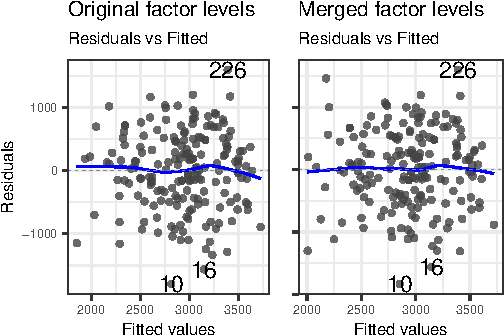
\includegraphics{Executive-Summary_files/figure-latex/residvfittedfull-1} 

}

\caption{Residuals vs Fitted values plot (Full model, post transformations)}\label{fig:residvfittedfull}
\end{figure}

\href{residvfittedfull}{Figure 3} shows no obvious non-linear pattern in
the residuals in either plot, with residuals approximately equally
distributed about 0, so our \textbf{linearity} and
\textbf{homoscedascity} assumptions were similarly satisfied.

\subsection{Model selection}\label{model-selection}

With our assumptions satisfied, we began stepwise variable selection to
construct models for each dataset, including only the most significant
predictors.

For each dataset, forward and backward selection procedures produced the
same models, with only \texttt{mother\ age}, and
\texttt{first\ trimester\ physician\ visits} dropped from the model.
This choice of selected predictors was further verified by an exhaustive
search - finding the same models for each dataset for the same number of
predictors.

The normality and independence assumptions for these newly constructed
models remained unchanged from the full models. Residual vs fitted
values plots (\href{figa1}{Figure A1}) were constructed to reassess our
linearity and homoscedascity assumptions, which were found to still be
satisfied.

\section{Results}\label{results}

\subsection{In-sample performance}\label{in-sample-performance}

\begin{table}[h]
  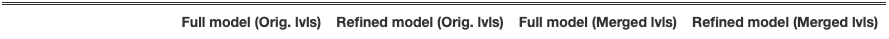
\includegraphics[width=0.5\textwidth, height=0.4cm]{titles}
  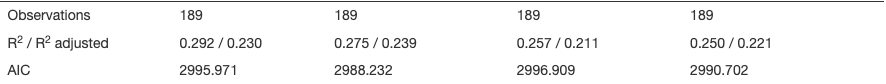
\includegraphics[width=0.5\textwidth, height=1.2cm]{results}
\caption{$R^2$ and AIC of each model}
\end{table}

\href{ll}{Table 2} shows the coefficient of determination, \(R^2\), was
highest in the model with the most predictors, and lowest in the model
with the least predictors. This was to be expected, as adding more
predictors to a model will always have a non-increasing effect on the
residual sum of squares.

Accordingly, the full model with the most number of predictors explained
the greatest proportion of variation within our results, giving it the
best in-sample performance.

However, this statistic alone tells us little about how the models
perform on unseen data, which the AIC attempts to account for by
penalising for more predictors, discouraging overfitting and hinting at
better out-of-sample performance.

We had significant reductions in AIC between each full model and its
refined alternative, indicating our refined models had better fit per
added predictor. Between the two refined models, the alternative with
original factor levels of premature labours had a marginally better AIC
by \textasciitilde2 points - making them approximately equally well
fitting.

An expanded version of \href{tb2}{Table 2} including model coefficients
can be found in the appendix, as \href{tba2}{Table A2}.

\subsection{Validating out of sample
performance}\label{validating-out-of-sample-performance}

To gauge out of sample performance, we performed 10-fold
cross-validation with 1000 repeats, with the results shown in
\href{fig4}{Figure 4}. Significant reductions in Root Mean Squared Error
and Mean Absolute Error that in our refined models, after dropping the
least significant predictors. Our models trained on the data with merged
factor levels also had better out of sample performance than those
trained on the original factor levels.

.

.

.

.

.

.

.

.

.

.

.

.

.

.

\subsection{Final model and
interpretation}\label{final-model-and-interpretation}

In choosing our final model, we prioritised out of sample performance to
allow to optimise for generalisability to future observations, whilst
also balancing for reasonable in-sample performance. Accordingly, we
chose the refined model with merged factor levels - having the best out
of sample performance at minimal cost to \(R^2\):

\begin{small}
\begin{flalign*}
& \widehat{\textcolor{blue}{\text{Birth weight}}} = 610.22 + 132.66(\operatorname{\textcolor{blue}{Race}}_{\operatorname{Other}}) + 460.01(\operatorname{\textcolor{blue}{Race}}_{\operatorname{White}}) \\ &-  316.87(\operatorname{\textcolor{blue}{Smoke}}_{\operatorname{Yes}}) - 211.68(\operatorname{\textcolor{blue}{PTL}}_{\operatorname{>=\ 1}}) - 562.41(\operatorname{\textcolor{blue}{HT}}_{\operatorname{Yes}}) \\ &- 483.45(\operatorname{\textcolor{blue}{UI}}_{\operatorname{Yes}}) + 572.37(\operatorname{\textcolor{blue}{\log(LMW)}})
\end{flalign*}
\end{small}

Holding all other predictors constant, mothers of ``other'' and
``white'' race had positive correlations with birth weight in comparison
to black mothers, whereas histories of smoking, premature labour/s,
hypertension, and uterine irritation were negatively correlated with
birth weight.

On average, a one percent increase in weight at last menstruation would
be expected to result in a 5.7 gram increase in weight at birth.

\subsection{Discussion and conclusion}\label{discussion-and-conclusion}

At the cost of avoiding overfitting, we merged factor levels in the
number of premature labour \& number of first trimester physician
visits, resulting in a loss of information. This contributes to a
limitation of our analysis, since our model is blind to any differences
from observations larger than our unique categories. This possibly
introduces bias and limits the model's predictive capacity.

Our data is only collected from one US medical centre, which is not a
representative sample of the wider population. This induces selection
bias, and the observations may not generalise well to other populations.

To overcome both of these limitations, more data collection is required.
A random sample with more observations would provide us with more
information, possibly reducing the necessity of merging factor levels.
It would also reduce selection bias, and provide better overall model
predictions.

In summary, there was a significant improvement in accuracy and a
decrease in errors for out of sample performance when we used our
refined model with merged factor levels. This was sufficiently balanced,
at the worthwhile expense of a slightly smaller \(R^2\) value. We also
found that the variables of mother's age and number of physician visits
were not very informative predictors for birth weight and hence could be
dropped from the regression model entirely.

%\showmatmethods


\bibliography{pinp}
\bibliographystyle{jss}



\end{document}
